% status: 0
% chapter: TBD

\title{Kubernetes and Containers}
\author{Bruce Walker}

%\affaddr{Phoenix, AZ}
%\email{brucwalk@iu.edu}
 
\date{ April 27, 2018}

\maketitle 
\section{Abstract}

Orchestration is the new buzz word in organizational infrastructure.
Companies are changing how they view and use applications.  The days
of large, cumbersome applications, spread over the entire
organization, are numbered.  A method of
managing applications and information, from the smallest of local 
office needs, to the largest of corporate needs, with much less 
overhead than traditional applications was needed.  Kubernetes is that 
platform.  



\section{Introduction}

There are many ways for organizations to structure their information
technology environments.  Traditional methods would include software
developers creating a large application and deploying it over the
organiztion. It could have been deployed via a server or locally on
any number of machines.  That is changing.  Kubernetes is fast 
becoming the most influential orchestration platform that
many have never heard of.  A recent development, it features power and
flexibility to ensure a place in the future of cloud computing.
Developed by Google, Kubernetes is a relatively new technology.  It
started in 2014 as an open source method of deploying and operating
application containers.  Google had a long history of developing
clusters and deploying applications on those clusters.  The resulting
application, Kubernetes, allowed management of large clusters. It is
a robust collection of processes, that are fast and dependable.  It is
scaleable and adaptive. Kubernetes is a container orchestration
application, that can run in a variety of environment.  It essentially
uses API's to describe and manage what applications are running in a 
container~\cite{concept}.

\begin{figure}[!ht]
\centering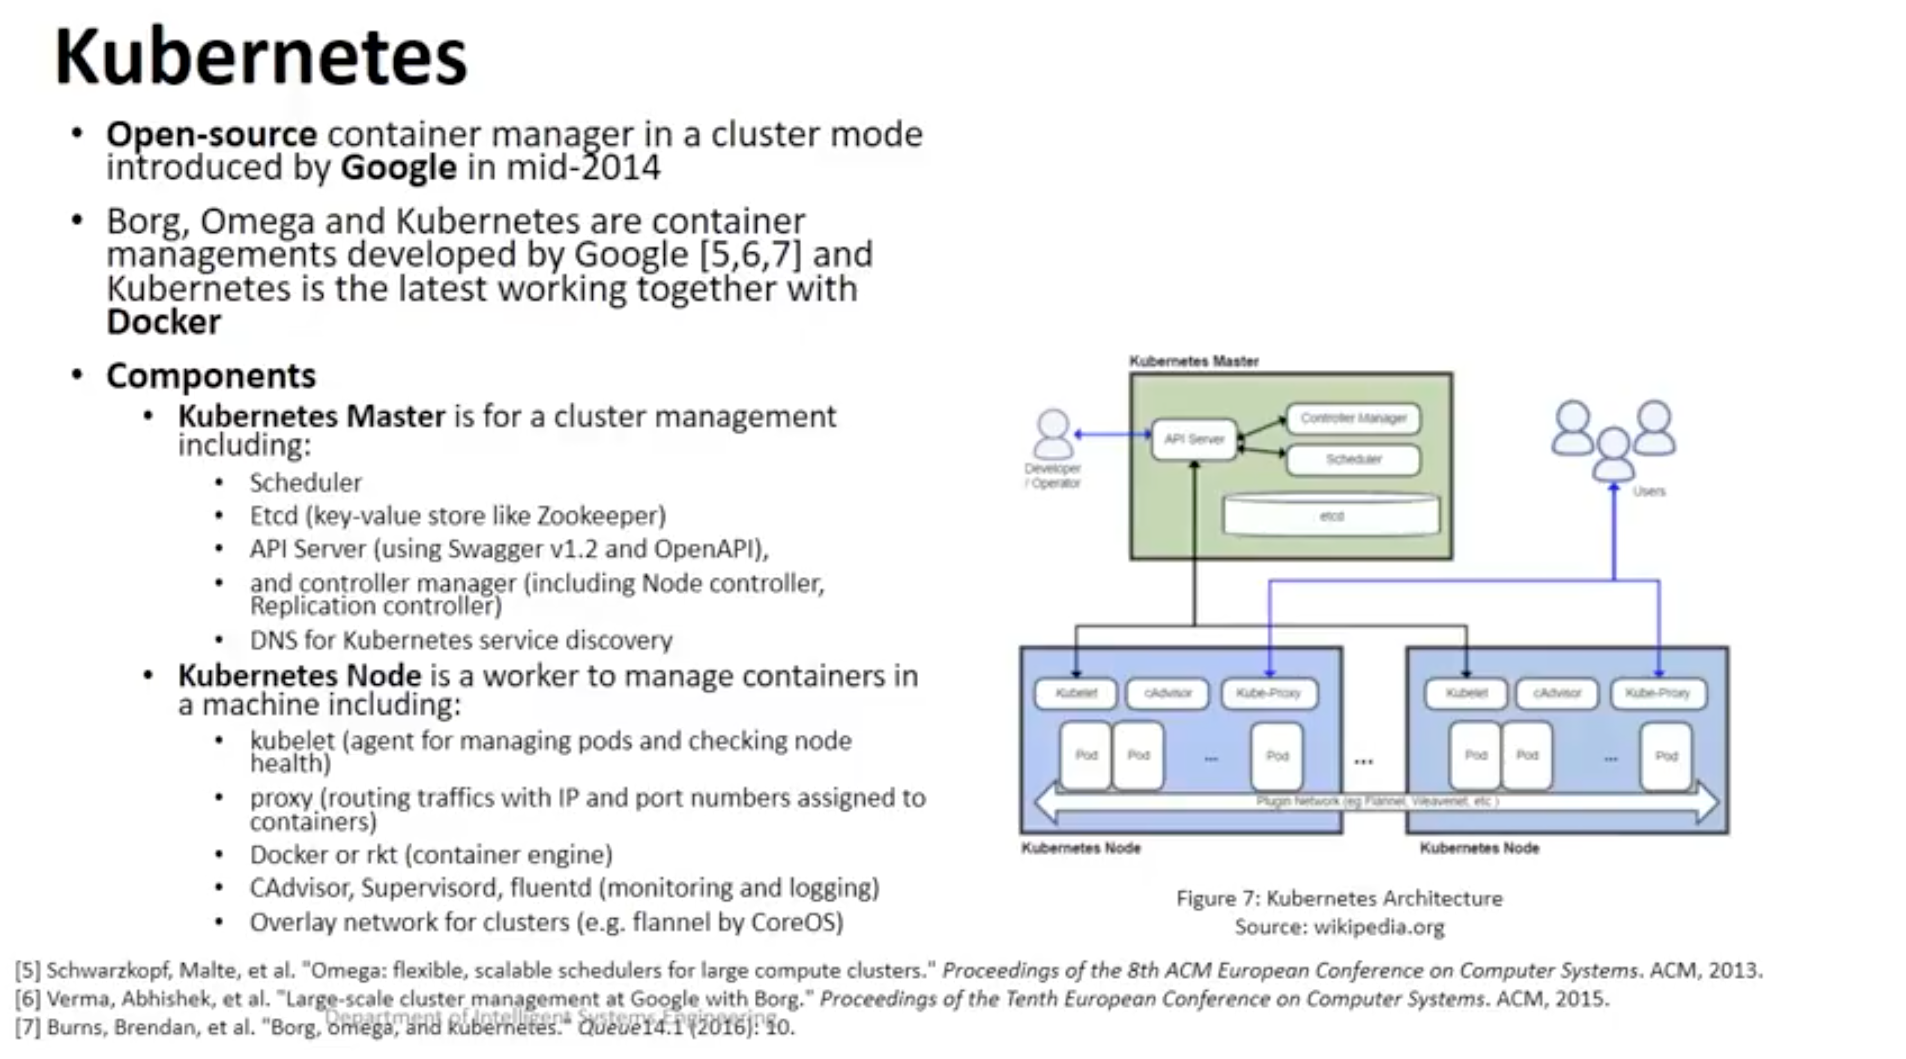
\includegraphics[width=\columnwidth]{images/kubernetes.png }~\cite{definition}.
\end{figure}

\section{How it Works}

 
Based on the success of Google's research, Kubernetes was launched as
an open source application.  From its inception, methods of computing 
and computing applications have moved from large applications to VM's
to Containers.  Historically, applications on computers or servers, require
large operating systems, that encompass the entire computer and
require that every application be subject to their commands.  Should
the operating system fail, all applications on the computer will also
fail.   

Kubernetes is different.  Essentially, it is a Container environment,
and microservices environment, and a cloud environment.  It can run on
a laptop or desktop.  It is just as ready to run on a virtual machine
in the cloud or even on bare metal servers.  Kubernetes uses its
systems like an operating system, except in smaller pieces of
applications at one time.  All of those pieces can be singularly run
or all run simultaneously.  When a piece of Kubernetes, other parts of
Kubernetes automatically step in and continue activity, if the user
requires that redundancy.\cite{concept}.

Kubernetes has three primary levels.  First, is the Pod.  It is the
building block for Kubernetes.  A single Pod is like a cell.  It can
be set up to receive a a Container of information.  In order to
receive that container, it must be configured.  Its memory must be
configured, to determine the amount of memory to allocated to it
\cite{pods}.  A Pod may hold one or more Containers.  A Pod has a
memory limit.  The Container or Containers assigned to the Pod also
have memory limits.  The Pod cannot comsume more memory than the
memory in the Container.  Pods are very versitile.  They can contain
and run an almost endless number and variety of applications.  The Pod
and the Container therein, must communicate with each other.  The
communication is accomplished via API.  The Pod is configured, at
creation or upon repupose, with downwardAPI Pods do not have to exist
in a singularfashion.  They can be clustered together to assigned to a Node.  

Thereafter, each Pod is assigned to a node.  A node can contain many
Pods.  Each Pod can contain one element or object necessary for the
entire Node to function, or an entire application can be contained
within a Pod.  Pods are scaleable.  

Kubernetes has eight primary features, although it has numerous other 
featuresand functions.

\begin{figure}[!ht]
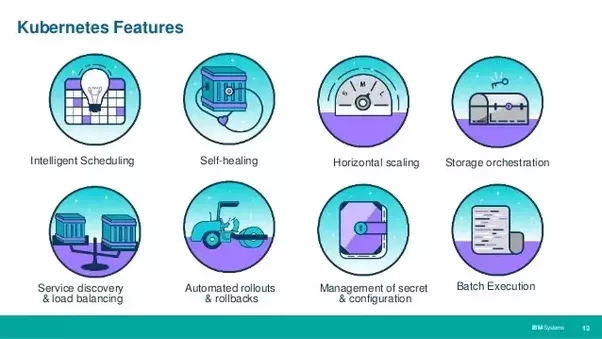
\includegraphics[width=\columnwidth]{images/features1.png}
\end{figure}

Kubernetes is a combination of numerous services.  It is a large scale
computing platform, while it also performs microservices.  It is
Platform as a Service (PaaS), while it is also not a PaaS. 

Once a determination is made on what platform on which to run
Kubernetes, configuring the right solution is next.  On the virtual 
machine, Kubernetes is installed by accessing an
outside site, like the Kubernetes site, to download the application.  There a
number of options, when it comes to which application to install.
Part of the variation is due to the particular version of virtual
machine used to run Kubernetes.  Also, the use of a more convenient,
and lighter form of Kubernetes, called Minikube is often used for a
virtual machine, such as Ubuntu\cite{minikube}. However, installation
is available for practically every platform, from Linux, to MacOS, to
Windows, and cloud platform, including Microsoft Azure, Amazon AWS,
even IBM, and others\cite{concept}.
It is a fast download and can access other Kubernetes options and
APIs.  Even though it is local, it can still
support\cite{concept}:

\begin{itemize}
    \item DNS 
    
    \item NodePorts 
    
    \item ConfigMaps and Secrets 
    
    \item Dashboards, Container 
    
    \item Runtime:  Docker, rkt, and CRI-O 
    
    \item Container Network Interface
    
    \item Ingress  
 \end{itemize}   
 
Once Kubernetes is installed on the virtual machine, it can be
deployed.  Kubernetes must be configured in order to properly deploy
and, for it to accept containers.  Once deployed, containers, with
applications can be layered on top of Kubernetes.  Kubernetes can then
create instances of the application ~\cite{concept}.

A cloud based option for available for Kubernetes use.  Cloud services 
have joined in using Kubernetes due to the reliability and ability to
offer a wide variety of services to customers.   

Since Kubernetes, and thus MiniKube, are similar to stand alone
machines, many aspects of their performance and behavior must be
configured.  The environment must be prepared, at drivers must be 
imported.  Minikube supports Kubernetes
features, such as DNS, NodePorts, ConfigMaps and Secrets, etc.   

\section{How to Get Started}

As mentioned earlier, downloading Kubernetes is accomplished by
visiting the Kubernetes site or utilizing the command line to access
Kubernetes versions, for laptops, desktops, and virtual machines.  

One method of utilizing the command line involves using the command
line tool kubectl.  Since Kubernetes is available on so many
platforms, the kubectl commands vary, slightly.  With Ubuntu, is
packaged as a snap application ~\cite{kubectl}.  Each platform has
its own version of the kbectl install package.  macOS installs via
Homebrew.  Windows installs via Powershell Gallery or Chocolatey.
Kuberntetes is also available via Goggle Cloud SDK\cite{kubectl}.\

Then comes the time to configure kubectl, so that it will connect to a
Kubernetes cluster.  The clustering aspect of Kubernetes is one of its
most important features.  A small machine can minic a large machine
with clustering\cite{kubectl}.  

Once a Pod or Node is configured, almost any application that can be
run on any computer, can run on a Kubernetes cluster.  The Container
can havae commands and arguments defined, when the Pod is created.
Data can then be passed into the Pod and Container.  Files can be
passed into the Container.  Even security credentials are used in Pods
and Containers.  Applications can be accessed via a web user
interface, as well as with the command line.  A Dashboard user
interface is available with graphics depicting the state of Pods and
Nodes and Services\cite{dash}.


\section{How Kubernetes is Used}

Kubernetes is used to perform the exact same functions that any other
computing system does.  Kubernetes does so with less computing
overhead and more flexibility, however\cite{dash}.  Utilizing the
operating system of the host means much less resource use than a
virtual machine, which requires an entire operating system to engage
when the virtual machine starts ~\cite{reasons}.  Containers are very
good at running internal functions and APIs, they are not generally
good at managing numerous Containers scattered around the office or
the globe.  This is where Kubernetes is most useful.  Kubernetes
excels at deploying and scaling Containers and their applications.  It
can ensure even workloads across the clusters ~\cite{reasons}.  In the
current software environment, applications are tasked to run on VMs,
bare metal, on premise servers, and cloud.  Designing a one size fits
all application is near impossible, but Kubernetes allows for
application development that can operate in any environment, due to
containerized operations ~\cite{reasons}.  

Applications are becoming modular.  That is, they are designed in
pieces, which fit into any platform, creating the same function, with
less overhead.  

Kubernetes has a hierarchical design.  At the lowest level are Pods.
Generally, Pods are where application containers are placed.  Pods are
the smallest units in the Kubernetes universe.  It essentially acts as
a host for application containers.  Pods can be closely linked, where
a single Pod will contain information, and a different Pod will
contain other information.  The Pods may or may not communicate with
each other.  The can be linked via API, if they need to
communicate.   

The next level of architecture is the Node.  All Pods run on a Node.
The Node is where much of the actual computing occurs.  A Node may be
physically located on a machine or it may be virtual or cloud
based. The Node allocates the resources needed by the Pods on a
machine.  A Node has a minimum level of processes that it must
perform.  It must run the Kubelet, which orchestrates Node and the
highest level, the Master level.  The Node must also run the what is
in the container.  The container application, Docker, for example is
managed by the Node.  It retrieves the container image from the
registry and then opens the application in the container.  Thereafter,
it runs the application. 

The Kubectl is the heart of Pod interactions.  It shows and details
resources and can execute commands and print logs from the Pod. 

Each Pod is a self contained environment, which requires authorization
and or proxy to access.  No alteration of the Pod can take place until
the kubectl proxy command is executed, in a separate terminal window.   
 


Kubernetes is deployed in a number of ways.  That number is
increasing, especially when cloud services are included.  On a local
machine, Kubernetes is deployed on a host machine and or on a virtual
machine, such as Ubuntu.  On the local machine, Kubernetes can be
deployed via the command line, using the following commands: 


On the virtual machine, deployment can occur through VirtualBox or
other VM.  The host operating system may require a BIOS update to
ensure the proper virtualization settings.   

Deploying Kubernetes to support a Docker environment is very popular.
Kubernetes can manage the Docker containers via a Kubernetes Service.
The service establishes policies that manage who has access to Pods.
This is referred to as a microservice.  Kubernetes services ensure a
high, overall level of reliability.  When Pods fail, their functions
are continued by replication controllers ensure that sufficient Pods
are available to perform as needed, without failure.  When a Pod is
created, additional Pods maybe created, identically structured, in
order to ensure availability of Pod functions~\cite{service}.  

Kubernetes is able to run on desktop and virtual machines.  For
example, to run Kubernetes on a Mac, Kubernetes is installed.
Thereafter, a containerservice, such as Docker can be downloaded. 
Docker includes an option, for Mac, that includes Kubernetes.  The 
two applications complimenteach other~\cite{service}.  Until recently,
Kubernetes was actually required to run a large number of Docker
Containers.  This is changed, somewhat, with the introduction Docker
Swarm, which allows Docker to orchestrate containers in a way that is
similar to Kubernetes~\cite{services}.

Another approach taken by organizations is adopting Kubernetes to make
some infrastructure and services so inexpensive, that they can become
almost disposable.  If part of the system fails, other microservices
can automatically replace the failed parts~\cite{reasons}.  

Interestingly, however utilizing orchestration on a database is
difficult.  Databases are not interchangeable, and thus, a Kubernetes
setup does not work.  One solution is to run the database as usual, or
migrate the database to the cloud~\cite{reasons}.  A solution to the
problem has been resolved by the latest release of Kubernetes.  It
allows for StatefulSets, which means that every Pod will retain the
same network identity, even after it is restarted.  This is true even
if the Pod is tasked to a different machine~\cite{reasons}.  

The latest Kubernetes also allows for DaemonSets.  DaemonSets let the
user assign some Nodes to always run specific Pods, which allows the
running of a database.  It isn't perfect in that dynamic scheduling of
Pods, as in StatefulSets, but the ability to schedule Pods is very
helpful ~\cite{reasons}.

Some of the Kubernetes features give the user additional flexibility.  

\subsection{Horizontal Scaling}

Kubernetes is a container-based environment, with pods as its default 
unit. The Pods communicate with each other.  It allows for Horizontal
Pod Autoscaling, which automatically scales the number of Pods being
utilized, depending on user determined settings or automatic
settings~\cite{concept}. Scaling can increase deployment or decrease
deployment with simple commands or as an automated
function~\cite{concept}.

The Horizontal Pod Autoscaler is an API resource and a controller.  It
will adjust deployment in relation to the average CPU
utilization~\cite{concept}.  

\subsection{Service Discovery and Load Balancing}

Kubernetes offers Services, which allow object creation.  Creation of
a REST object resembles a Pod.  It can even be a TCP or UDP protocol.
In addition, Kubernetes capabilities include creation of virtual IPs
via a Node cluster.  No need to modify your application to use an
unfamiliar service discovery mechanism~\cite{concept}. Kubernetes
allows the user to specify an IP of their choice.  A DNS server is
also part of Kubernetes services.  Load Balancing of traffic is
included as part of Kubernetes services.  Load Balancing is also
available for Microsoft Azure and AWS~\cite{concept}.

\subsection{Self-healing}

Who

What  

When

where

Why

How


\subsection{Automated Rollouts and Rollbacks}

Kubernetes contains a deployment controller, which allows for Pod
creation.  It also allows for the creation of replicas of the most
recent configuration.  Deployments can be managed by use of the
command line.  New Pods can be set to replicate ~\cite{concept}. A
deployment can also be set to rollback, automatically~\cite{concept}.  

\subsection{Secret and Configuration Management}

Kubernetes features objects called ' 'secret,' ' which hold passwords,
tokens, ssh keys, and other sensitive information.  Users can create
secrets.  The system creates secrets, as well.  Some secrets are
included in Kubernetes~\cite{concept}.  Kubectl allows creation of
user names and password used by the Pod to authenticate the  
user~\cite{concept}.  

\subsection{Storage Orchestration}

Storage issues are addressed by Kubernetes.  PersistentVolume is part
of Kubernetes, and it is connected for users, by an API.  The API
allows the user to monitor the storage~\cite{concept}.  Storage is
both static and dynamic.  A cluster administrator determines the level
of PersistentVolume storage.  Dynamic storage is created by the
cluster if the static does not match a user's PersistentVolumeClaim.
Kubernetes supports a wide range of persistent volumes.    


\subsection{Batch Execution}

Kubernetes creates jobs to create Pods or to terminate Pods.  A job
configuration is completed to begin running the created
job~\cite{concept}.   




Kubernetes, and the applications it supports, are easily downloaded.
Upon downloading, Docker can be layered on top of Kubernetes.   

\section{Conclusion}

Kubernetes is a flexible, scaleable platform, which is perfectly
suited for today's application development.  It is a container
platform, and a microservices platform, and a cloud platform.  It
manages containers and orchestrates computing and networking, storage,
and infrastructure.  









\bibliographystyle{ACM-Reference-Format}
\bibliography{report}


